\documentclass[crop=false]{standalone}
\begin{document}
	\section{System Overview}
	
	在未來我們希望可以加入視覺感測器,例如:單目攝影機,雙目攝影機,深度攝影機,再搭配深度學習模型,例如 YOLO等物件偵測模型。使用視覺感測器捕捉畫面後,交由深度學習模型負責執行物件偵測,再模型偵測到的物件位置轉換座標系後給 DWA 動態調整路徑。並且可以加入最短路徑演算法,加速 DWA 在評選路徑時的速度。
	
	\begin{figure*}[thbp!]
		\centering
		\fbox{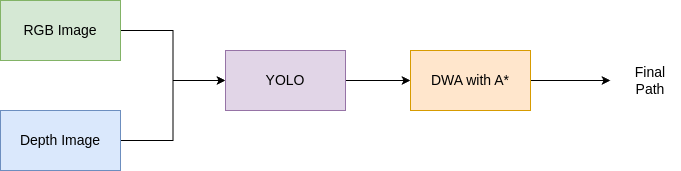
\includegraphics[width=\textwidth]{furtherwork_workflow}}
		\caption{The furtherwork workflow}
		\label{fig:furtherwork}
	\end{figure*}
\end{document}